% if you want the answers to appear uncomment the below
\documentclass[answers]{exam}
% otherwise uncomment the below
% \documentclass{exam}
\usepackage[bottom]{footmisc}
\usepackage{graphicx}
\usepackage[letterpaper, margin=.9in]{geometry}
\usepackage{natbib}
\bibpunct{(}{)}{;}{a}{,}{,}
\usepackage{url}
\def\UrlFont{\rm}


\usepackage{Sweave}

\usepackage[utf8x]{inputenc}
\usepackage{array}
\usepackage{verbatim}
\usepackage{amsfonts}
\usepackage{amsmath}
%\usepackage{lineno}
\setlength{\parskip}{2ex}
%\setlength{\parindent}{0ex}

% Cannot place floats in figure environment.
\usepackage{caption}
\usepackage{newfloat}
%\DeclareCaptionListFormat{myliststyle}{#1.#2}
\DeclareCaptionType{mytype}[Solution Fig.][List of mytype]
\newenvironment{myfigure}{\captionsetup{type=mytype}}{}



\newenvironment{packed_enum}{
\begin{enumerate}
 \setlength{\itemsep}{0pt}
  \setlength{\parskip}{0pt}
  \setlength{\parsep}{0pt}
}{\end{enumerate}}
\newenvironment{packed_item}{
\begin{itemize}
 \setlength{\itemsep}{0pt}
  \setlength{\parskip}{0pt}
  \setlength{\parsep}{0pt}
}{\end{itemize}}

 \newcommand\independent{\protect\mathpalette{\protect\independenT}{\perp}}
    \def\independenT#1#2{\mathrel{\setbox0\hbox{$#1#2$}%
    \copy0\kern-\wd0\mkern4mu\box0}}


\bibliographystyle{plainnat}

\pagestyle{myheadings}
\markright{Advanced Topics in Causal Inference \hfill  R Lab \#2 \hfill}


\title{R Lab 2 - Calculating True Values of Target Causal Parameters Under Longitudinal Interventions }
\author{Advanced Topics in Causal Inference}
\date{}

\begin{document}
\maketitle



\noindent \textbf{Assigned:} September 14, 2021\\
\textbf{Lab due:} September 21, 2021 on bCourses. Please answer all questions and include relevant \texttt{R} code. You are encouraged to discuss the assignment in groups, but should not copy code or interpretations verbatim. Upload your own completed lab to bCourses.


\noindent \textbf{Last lab:} \\
1. Explore different data structures, inspired by real-world experiments. \\
2. Simulate data generating systems that give rise to data we observe. \\
3. Think of studies in which these data generating systems may occur. \\


\noindent \textbf{Goals for this lab:} \\
Translate causal questions into target causal parameters and intervene on the Structural Causal Models (SCMs) to evaluate them.


\noindent \textbf{Next lab:}\\
Understand time dependent confounding and identifiability in a longitudinal context.



\begin{center}
\noindent\rule{18cm}{0.4pt}
\end{center}

\section{Introduction and Motivation}

In this lab, we're going to play with the ``root" of where data comes from to generate hypothetical outcomes that answer our causal questions.

\noindent In the previous lab, we learned how to simulate data generating systems that give rise to data we observe. Now, we're going to intervene on those data generating systems by deterministically setting certain variables to constant values (what kind of regime does this correspond to?), according to our ideal experiment/causal question of interest. After intervening, we'll generate many counterfactual outcomes. Then, we can apply a function to the distribution of those counterfactual outcomes, or more generally, to the post-intervention distribution of the data, (the function being $\Psi^F(P_{U,X})$) to evaluate the true value of our target causal parameter of interest that answers our causal question.

\noindent Note that it is also often possible to evaluate $\Psi^F(P_{U,X})$ analytically and obtain a closed-form solution. But, as mentioned in the previous lab, we can also turn to simulations to obtain answers computationally.


\begin{figure}
\begin{center}

\includegraphics[width=.5\textwidth]{target2.jpg}
\caption{Target parameter.}
\end{center}
\end{figure}

\section{This lab}

Recall that your GSR urgently needs you to determine whether lack of sleep is hurting students' academic performance and health. Also remember that we have perfect knowledge of how these outcomes come to be in the world, and more specifically, how they're impacted by sleep, background variables, and random error. In other words, unlike reality, we know the true data generating process.

\noindent We also have the power to intervene on these processes. For example, we can ``force" all students to get 8 hours of sleep -- would students' statistics test scores improve compared to if students got less than 8 hours of sleep? By how much? What about their probability of getting sick? How would the distribution of these outcomes differ if students got 8 or more hours of sleep for multiple nights in a row before the test? In this lab, based on the same 4 data structures as last lab, you'll come up with causal parameters and evaluate their true values (via simulations) to answer these causal questions.

\noindent Refer back to \texttt{R} Lab 1 for variable definitions and SCMs.



\subsection{To turn in:}


\noindent\fbox{
    \parbox{\textwidth}{

\textbf{\underline{For each of the 4 data structures listed below, answer the following questions:}} \\

\vspace{2mm}
\textit{\textbf{Note:}} For Data Structure 2, there are 2 causal questions. Go through the following steps for \textbf{both} causal questions.
\vspace{2mm}
\begin{enumerate}
\item \textbf{Write the causal target parameter that would answer the causal question posed using the data structure presented. What are the counterfactual outcomes?} Explain using notation and in words.
\item \textbf{Explain how to intervene on the SCM to get at the causal question/parameter of interest.} Refer back to \texttt{R} Lab 1 for each data structure's SCM.
%\item \textbf{Set the seed to 252.}
\item \textbf{Implement the intervention described in step 2} by updating the data generating function you created in \texttt{R} Lab 1.
\item \textbf{Evaluate $\Psi^F(P_{U,X})$ via simulated counterfactuals.} Given a large sample of counterfactual outcomes (say, $n = 100,000$), we can closely approximate $\Psi^F(P_{U,X})$.
\item \textbf{Write a sentence interpreting the value you got for $\Psi^F(P_{U,X})$.}
\end{enumerate}

    }
}

\pagebreak
\noindent\large\textbf{Data Structure 1: $O = (W, A, L, \Delta, \Delta Y)$}
\normalsize

\noindent \underline{Causal question:} What is the absolute difference in expected test score if all students slept 8 or more hours compared to if all students slept less than 8 hours, under a hypothetical intervention to ensure that everyone takes the statistics test?

\begin{enumerate}
\item \textbf{Write the causal target parameter. What are the counterfactual outcomes?} Explain using notation and in words.
\item \textbf{Explain how to intervene on the SCM to get at the causal question/parameter of interest.} Refer back to \texttt{R} Lab 1 for this data structure's SCM.
%\item \textbf{Set the seed to 252.}
\item \textbf{Implement the intervention described in step 2} by modifying the original data generating function created in \texttt{R} Lab 1. Call the new function \texttt{generate\_data1\_intervene}:
\begin{enumerate}
\item Copy and paste the data generating function (for this data structure) from \texttt{R} Lab 1, \texttt{generate\_data1()}.
\item In addition to the argument in your function specifying the number of observations you want to generate (i.e., $n$), add arguments to your function based on the variables you want to intervene on. For example, if you want to intervene on $A$, add an argument \texttt{a} to your function:
\begin{Schunk}
\begin{Sinput}
> generate_data_example = function(n, a) {  # add the argument "a"
+ 
+   U.W = rnorm(n, mean = 1, sd = 1)
+   U.A = runif(n, min = 0, max = 1)
+   U.Y = rnorm(n, mean = 1, sd = 3)
+ 
+   W = U.W
+   A = as.numeric(W + U.A < 1.5)
+   Y = W + A + U.Y
+ 
+   O = data.frame(W, A, Y)
+ 
+   return(O)
+ 
+ }
\end{Sinput}
\end{Schunk}
\item Intervene on the endogenous variables of interest by setting them equal to the new arguments you added in the previous step. For example, if you want to intervene on the random variable ``A" by setting it equal to the constant ``a", then set \texttt{A} equal to \texttt{a} within your function:
\begin{Schunk}
\begin{Sinput}
> generate_data_intervene_example = function(n, a) {
+ 
+   U.W = rnorm(n, mean = 1, sd = 1)
+   U.A = runif(n, min = 0, max = 1)
+   U.Y = rnorm(n, mean = 1, sd = 3)
+ 
+   W = U.W
+   A = a # intervention is on A, so set A equal to a
+   Y = W + A + U.Y
+ 
+   X = data.frame(W, A, Y)
+ 
+   return(X)
+ 
+ }
\end{Sinput}
\end{Schunk}
\end{enumerate}
\item \textbf{Evaluate $\Psi^F(P_{U,X})$}:
\begin{enumerate}
\item Generate 100,000 observations of the data generating system you intervened on. Remember to add the values you want to intervene with as arguments. Store this in a dataframe. For example:
\begin{Schunk}
\begin{Sinput}
> X_example1 = generate_data_intervene_example(n = 100000, a = 1) # setting A = 1
\end{Sinput}
\end{Schunk}
\item Extract the outcome(s) from the dataframe you generated in the previous step. These are your counterfactual outcomes. Remember that one way to extract a variable from a dataframe is using the dollar sign, \texttt{\$}. For example:
\begin{Schunk}
\begin{Sinput}
> X_example1$Y # here we are extracting the counterfactual outcome Y1 from X_example1
\end{Sinput}
\end{Schunk}
\item Evaluate $\Psi^F(P_{U,X})$ using the simulated counterfactual outcomes to obtain the true value of your target causal parameter. \textit{Hint: take the mean of both counterfactual outcomes from the previous step, and subtract (in the right direction)!}
\end{enumerate}
\item \textbf{Interpret $\Psi^F(P_{U,X})$.}
\end{enumerate}


\noindent\large\textbf{Data Structure 2: $O = (L(1), A(1), L(2), A(2), L(3), A(3), L(4), A(4), Y)$}
\normalsize

\noindent\underline{Causal question 1:} How would the expected exam score at the end of the study (i.e., after $t=4$ days) have differed if all students got 8 or more hours of sleep every night during the entire study (i.e., at $t=1,2,3,4$ days) versus if all students got less than 8 hours of sleep every night during the entire study (i.e., at $t=1,2,3,4$ days)?


\begin{enumerate}
\item \textbf{Write the causal parameter that would answer Causal question 1. What are the counterfactual outcomes?} Explain using notation and in words.
\item \textbf{Explain how to intervene on the SCM to get at Causal question 1.} Refer back to \texttt{R} Lab 1 for this data structure's SCM.
%\item \textbf{Set the seed to 252.}
\item \textbf{Implement the intervention you described in step 2} by modifying \texttt{generate\_data2()} from the previous lab. Call the new function \texttt{generate\_data2\_intervene}.
\begin{enumerate}
\item Similar to the previous data structure, copy the function \texttt{generate\_data2()} from \texttt{R} Lab 1 and add an argument to the function that takes in \textit{a vector} of values you want to intervene with. Name that vector \texttt{abar}.
\item Intervene on the endogenous variables of interest by setting them equal to the \textit{position} of the vector you added in the previous step. Use brackets to subset by position the value of interest from the vector \texttt{abar}. Adding to the previous example, if you want to set $A(1) = a(1)$ and $A(2) = a(2)$:
\begin{Schunk}
\begin{Sinput}
> generate_data_intervene_example2 = function(n, abar) {
+ 
+   U.W = rnorm(n, mean = 1, sd = 1)
+   U.A1 = runif(n, min = 0, max = 1)
+   U.A2 = runif(n, min = 0, max = 1)
+   U.Y = rnorm(n, mean = 1, sd = 3)
+ 
+   W = U.W
+   A1 = abar[1] # subset first position of abar vector to set equal to a(1)
+   A2 = abar[2] # subset second position of abar vector to set equal to a(2)
+   Y = W + A1 + A2 + U.Y
+ 
+   X = data.frame(W, A1, A2, Y)
+ 
+   return(X)
+ 
+ }
\end{Sinput}
\end{Schunk}
\end{enumerate}
\item \textbf{Evaluate $\Psi^F(P_{U,X})$}.
\begin{enumerate}
\item Generate 100,000 observations of the data generating system you intervened on. Remember to add the vector of values you want to intervene with, \texttt{abar} as an argument. Store this in a dataframe.
\begin{Schunk}
\begin{Sinput}
> # setting A1 = 0 and A2 = 0
> X_example2 = generate_data_intervene_example2(n = 100000, abar = c(0, 0))
\end{Sinput}
\end{Schunk}
\item Extract the simulated counterfactual outcomes from the dataframe (as was done in the previous data structure) and evaluate $\Psi^F(P_{U,X})$.
\end{enumerate}
\item \textbf{Interpret.}
\end{enumerate}



\vspace{4mm}
\noindent \underline{Causal question 2:} How does cumulative days getting 8 or more hours of sleep affect students' statistics exam scores at the end of the study? Specifically, say you are willing to assume a linear relationship between total number of days on which a student got 8 or more hours of sleep and expected exam score. How could you summarize how much the expected exam score would change per additional night on which a student got at least 8 hours of sleep?

\begin{enumerate}
\item \textbf{Write the causal parameter that answers Causal question 2.} \textit{Hint: refer to 252E Lecture 1, slides titled: ``Defining target parameters using a longitudinal marginal structural model."}
\item \textbf{Explain how to intervene on the SCM to answer Causal question 2.} Refer back to \texttt{R} Lab 1 for this data structure's SCM. \textit{Hint: instead of only setting $\bar{A}(4)=1$ or $\bar{A}(4)=0$, list out \underline{all} the possible ways we could intervene on this SCM (i.e., every possible $\bar{a}(4)$).}
%\item \textbf{Set the seed to 252.}
\item \textbf{Implement the intervention.}\\
\emph{Hint: Use the exact same function as Causal question 1,} \texttt{generate\_data2\_intervene()}\emph{, to intervene! Skip to the next question.}
\item \textbf{Evaluate $\Psi^F(P_{U,X})$.} For each possible sleep regime $\bar{a}(4)$, calculate the corresponding expected test score under that regime $E[Y_{\bar{a}}]$. Summarize these expected outcomes as a linear function of total number of nights with 8 or more hours of sleep. %What are the possible number of times a student could get 8 or more hours of sleep out of 4 nights? What are the possible sleep regimes (i.e., values of $\bar{a}(4)$) that would result in each possible total number of nights with 8 or more hours of sleep?
\begin{enumerate}
\item Make a matrix of all 16 possible $\bar{a}(4)$ regimes, where each row is a single regime and column is $A(1), ..., A(4)$.
\begin{itemize}
\item[] \textit{Hint:} Use the the \texttt{expand.grid()} function, which takes in a vector and creates a data frame with all the possible permutations of the elements in that vector. Use the \texttt{colnames()} function to name the columns of matrix of $\bar{a}(4)$ permutations:
\begin{Schunk}
\begin{Sinput}
> # matrix of every possible abar permutation
> abar_mat = expand.grid(c(0,1), c(0,1), c(0,1), c(0,1))
> # make column names each intervention node
> colnames(abar_mat) = c("A1", "A2", "A3", "A4")
\end{Sinput}
\end{Schunk}
\end{itemize}
\item Create two new vectors of length 16 filled with \texttt{NA}s called \texttt{sum.abar} and \texttt{EY.abar}. In the next step, we will populate \texttt{sum.abar} with each regime's cumulative treatment and \texttt{EY.abar} with each regime's expected counterfactual outcome.
\item Create a \texttt{for} loop to compute the expected counterfactual outcome for each treatment regime. Recall that this is the syntax to create a for loop from \texttt{i} in \texttt{1:n}:
\begin{Schunk}
\begin{Sinput}
> for (i in 1:n) {
+   # insert code within for loop here
+ }
\end{Sinput}
\end{Schunk}
Within a for loop from \texttt{i} in \texttt{1:16}, do the following:
\begin{enumerate}
\item Generate a new data frame in which $\bar{A}(4)$ is intervened on using the $i^{th}$ treatment regime in the \texttt{abar\_mat} matrix.
\begin{itemize}
\item[] \textit{Hint:} Use the \texttt{generate\_data2\_intervene()} function to generate the new, intervened-on data, with the \texttt{abar} argument equal to the $i^{th}$ row of \texttt{abar\_mat}. Set this new data equal to \texttt{X}:
\begin{Schunk}
\begin{Sinput}
> X = generate_data2_intervene(n = 100000, abar = as.numeric(abar_mat[i,]))
\end{Sinput}
\end{Schunk}
\end{itemize}
\item Get the cumulative treatment for the $i^{th}$ regime, and save it to the $i^{th}$ row of \texttt{sum.abar}.
\begin{itemize}
\item[] \textit{Hint:} Use the \texttt{rowSums} function on the $i^{th}$ regime in \texttt{abar\_mat}. Save this cumulative treatment to the $i^{th}$ position of the \texttt{sum.abar} vector:
\begin{Schunk}
\begin{Sinput}
> sum.abar[i] = rowSums(abar_mat)[i]
\end{Sinput}
\end{Schunk}
\end{itemize}
\item Get the mean counterfactual outcome under $i^{th}$ regime, and save it in the $\texttt{i}^{th}$ position of \texttt{EY.abar}:
\begin{Schunk}
\begin{Sinput}
> EY.abar[i] = mean(X$Y)
\end{Sinput}
\end{Schunk}
\end{enumerate}
\end{enumerate}

\noindent\fbox{
    \parbox{\textwidth}{
\textit{Pause here: what did we just do?}
\begin{itemize}
\item[-] For each of the 16 possible treatment regimes $\bar{a}(4)$ (stored in \texttt{abar\_mat}), we got the expected counterfactual outcome $E[Y_{\bar{a}}]$ (stored in \texttt{EY.abar}) under that regime.
\item[-] We also have a corresponding summary measure (in this case, a simple sum) of each treatment regime ($\sum\bar{a}(4)$, stored in \texttt{sum.abar}).
\end{itemize}
}
}
\item \textbf{Evaluate $\Psi^F(P_{U,X})$.}  Recall that we are assuming that the expected outcome under each treatment regime $E[Y_{\bar{a}}]$ varies as a linear function of cumulative treatment $\sum\bar{a}(4)$. Use the \texttt{glm()} function to obtain the coefficients of this linear fit.
\item \textbf{Interpret $\Psi^F(P_{U,X})$}. Recall that our causal question of interest is: ``how much does the expected exam score change per additional night on which a student got at least 8 hours of sleep?" Which coefficient from the previous step answers this question?
\item \textbf{Bonus:} Is the linear MSM you wrote down correctly specified? Why or why not? If you are not willing to assume that your MSM is correctly specified, but you are still interested in a linear summary of how the expected counterfactual exam score varies as a function of cumulative number of nights on which a student got more than 8 hours of sleep, how would you modify your target parameter?
\item \textbf{Extra bonus!} Plot the true underlying values $E[Y_{\bar{a}}]$ for each $\bar{a}$ and their projection onto the linear working model.
\end{enumerate}





\begin{solution}
\noindent\underline{Causal question 2}


1. We will use a Marginal Structural Model (MSM) to help us answer this question:

\[
\Psi^F(P_{U,X}) = m(\bar{a}|\beta) = E[Y_{\bar{a}}] = \beta_0 + \beta_1 \sum_{t=1}^4a(t)
\]

This MSM lets us summarize how the expectation of counterfactual statistics test scores varies as a function of cumulative sleep. In particular, we are interested in $\beta_1$ as it will tell us how the above summary measure (total number of full nights of sleep) affects the outcome (i.e., for one additional night of 8 or more hours of sleep, what is the change in students' mean counterfactual test score?).

As written above, we are assuming a correctly specified MSM. In practice, we generally can't assume that the MSM is correctly specified, so we use a working MSM, and instead, the above parameter, $\beta$, gives us the projection of the true ``causal curve" $E_{U,X}[Y_{\bar{a}}]$, for all possible $\bar{a}$ onto a linear summary model, $m(\bar{a}|\beta)$ (see the bonus question).

2. We would use the same intervention on our SCM; however, instead of setting $\bar{A}(4) = 1$, then $\bar{A}(4)=0$, we would need to intervene to generate every possible $\bar{a}(4)$. That is:
\begin{align*}
a(1) & = 0, a(2) = 0, a(3) = 0, a(4) = 0 \\
a(1) & = 1, a(2) = 0, a(3) = 0, a(4) = 0 \\
a(1) & = 0, a(2) = 1, a(3) = 0, a(4) = 0 \\
& ... \\
a(1) & = 1, a(2) = 1, a(3) = 1, a(4) = 1
\end{align*}

There are $2^{4} = 16$ possible permutations of $\bar{a}(4)$.


3. We will use the same function as Causal question 1 (above) to intervene.

\begin{Schunk}
\begin{Sinput}
> #4. evaluate Psi.F
> # matrix of every possible txt regime permutation
> # Each column is an intervention at time t, or A(t).
> # Each row is a possible instance of abar.
> abar_mat = expand.grid(c(0,1), c(0,1), c(0,1), c(0,1))
> # name the columns
> colnames(abar_mat) = c("A1", "A2", "A3", "A4")
\end{Sinput}
\end{Schunk}
\begin{Schunk}
\begin{Sinput}
> # create an empty vector of NAs for the cumulative abars and mean counterfactual outcomes
> sum.abar = EY.abar = rep(NA, 16)
\end{Sinput}
\end{Schunk}
\begin{Schunk}
\begin{Sinput}
> # "For" loop to generate counterfactual outcomes.
> # For every rows of the dataframe of possible a(t)'s, apply the function
> # generate_data2_intervene() to generate data that has
> # been intervened on with that abar regime.
> # Take the mean of the Y's of interest.
> for(i in 1:16) {
+ 
+   X = generate_data2_intervene(100000, abar = as.numeric(abar_mat[i,]))
+   sum.abar[i] = rowSums(abar_mat)[i]
+   EY.abar[i] = mean(X$Y)
+ 
+ }
\end{Sinput}
\end{Schunk}
\begin{Schunk}
\begin{Sinput}
> # use ordinary least squares regression to obtain beta coefficients.
> # the target parameter is the coefficient value that minimize the L2 risk function
> MSM = glm(EY.abar ~ sum.abar)
> MSM
\end{Sinput}
\begin{Soutput}
Call:  glm(formula = EY.abar ~ sum.abar)

Coefficients:
(Intercept)     sum.abar  
     58.019        3.391  

Degrees of Freedom: 15 Total (i.e. Null);  14 Residual
Null Deviance:	    264.5 
Residual Deviance: 80.59 	AIC: 77.27
\end{Soutput}
\begin{Sinput}
> # beta 1 coefficient
> TrueMSMbeta1 = MSM$coefficients[[2]]
> TrueMSMbeta1
\end{Sinput}
\begin{Soutput}
[1] 3.390664
\end{Soutput}
\end{Schunk}


5. The true dose-response curve's intercept is 58.019 and slope is 3.391. This means that, if we believe this MSM is correct, cumulative days with 8 more hours of sleep has a positive linear effect on the mean counterfactual statistics test scores. For one more night of 8 or more hours of sleep, students' statistics test scores increase by 3.391 points, on average.

\vspace{2mm}

\textbf{Bonus:} The linear MSM we wrote down is not correctly specified. To see why not, note that even though the $A$ at each time point has the same direct effect on $Y$, an intervention on $A(1)$ will have a different effect on $Y$ than an intervention on $A(4)$, because an intervention on $A(1)$ will also affect $Y$ via its effects on intervening $L$'s.

We could modify our target parameter by defining a \textit{working} MSM, in which the target parameter $\beta$ is defined as a projection of the true underlying causal curve $E_{U,X}(Y_a)$ onto a linear working model $m(a|\beta)$:

\begin{align*}
\beta(P_{U,X} | m) &= argmin_{\beta} \ E_{U,X}\left[ \sum_{\bar{a}\in \mathcal{A}} \big(Y_{\bar{a}} - m(\bar{a} | \beta)\big)^2 \right] \\
m(\bar{a} |\beta) &= \beta_0 + \beta_1 \sum_{t=1}^4 a(t)
\end{align*}

Thus, projecting the causal dose-response curve onto the working MSM yields coefficients of $\beta_0 = $ 58.019 and $\beta_1= $ 3.391. In other words, summarizing the true causal dose-response curve with a linear working MSM suggests that cumulative sleep has a positive linear effect on mean statistics exam score.

\noindent \textit{Extra: MSM with different projection function}

We can modify the working MSM further by using a projection function, $g_n(\bar{A}(K))$ (i.e., the marginal probability of receiving each treatment regime of interest). Adding stabilized weights allows for weaker positivity assumptions -- the target parameter is still defined if some regimes don't occur. When we stabilize, however, we are working with a different causal parameter than without stabilization.

To do this, we will need to generate a large number of observations from data generating system 2 \textit{without} intervening on the system, and calculate the marginal probability of each of the 16 observed treatment regimes. We will repeat our regression of $E[Y_{\bar{a}}]$ for each possible $\bar{a}$ on the linear MSM, but now we will fit a weighted linear regression, where each $E[Y_{\bar{a}}]$ gets a weight corresponding to its probability of occuring in the observed data.


\begin{Schunk}
\begin{Sinput}
> # generate a large number of observations
> ObsData2 = generate_data2(n=100000)
\end{Sinput}
\end{Schunk}
\begin{Schunk}
\begin{Sinput}
> # initialize a vector for the marginal probability of each permutation of abar(4)
> # in other words, g(abar(4))
> g.abar = rep(NA, 16)
\end{Sinput}
\end{Schunk}
\begin{Schunk}
\begin{Sinput}
> # calculate the marginal probability of each of the 16 observed treatment regimes
> for(i in 1:16){
+   # marginal probability
+   marg.prob = mean(ObsData2$A1 == abar_mat[i,1] &
+                      ObsData2$A2 == abar_mat[i,2] &
+                      ObsData2$A3 == abar_mat[i,3] &
+                      ObsData2$A4 == abar_mat[i,4])
+   # assign to subject in vector g.abar
+   g.abar[i] = marg.prob
+ }
\end{Sinput}
\end{Schunk}
\begin{Schunk}
\begin{Sinput}
> # run the regression E[Yabar] on sum of abar, with new weights
> MSM_wts = glm(EY.abar ~ sum.abar, weights = g.abar)
> MSM_wts
\end{Sinput}
\begin{Soutput}
Call:  glm(formula = EY.abar ~ sum.abar, weights = g.abar)

Coefficients:
(Intercept)     sum.abar  
     58.003        3.395  

Degrees of Freedom: 15 Total (i.e. Null);  14 Residual
Null Deviance:	    16.53 
Residual Deviance: 5.045 	AIC: 77.3
\end{Soutput}
\begin{Sinput}
> # beta1 coefficient
> TrueMSMbeta1_wts = MSM_wts$coefficients[[2]]
> TrueMSMbeta1_wts
\end{Sinput}
\begin{Soutput}
[1] 3.394781
\end{Soutput}
\end{Schunk}


Now, the true dose-response curve's slope is 3.395. This means that, if we believe this MSM is correct, cumulative days with 8 more hours of sleep has a positive linear effect on the mean counterfactual statistics test scores. For one more night of 8 or more hours of sleep, students' statistics test scores increase by 3.395 points, on average.



\textbf{Extra bonus!}



\begin{Schunk}
\begin{Sinput}
> # plot the expected test score as a function of cumulative sleep (unweighted)
> plot(sum.abar, EY.abar,
+      main='Expected counterfactual test score as a function of cumulative sleep',
+      xlab='Days with 8 or more hours of sleep',
+      ylab='Expected counterfactual test score',
+      pch = 16,
+      col=as.factor(EY.abar),
+      cex = .7)
\end{Sinput}
\end{Schunk}
\begin{Schunk}
\begin{Sinput}
> # add the true value of the causal parameter beta to the graph (in blue).
> abline(MSM, col='blue')
\end{Sinput}
\end{Schunk}
\begin{Schunk}
\begin{Sinput}
> # add the true causal curve (weighted) to the graph (in red).
> abline(MSM_wts, col = "red")
\end{Sinput}
\end{Schunk}
\begin{Schunk}
\begin{Sinput}
> # add legend
> legend("topleft",
+        legend = c("True MSM with 1 as proj. function", "True MSM with marg. prob of regime \n as proj. function"),
+        col = c("blue", "red"),
+        lty = 1,
+        text.font=2,
+        box.lty=0)
\end{Sinput}
\end{Schunk}

\begin{myfigure}
\begin{center}
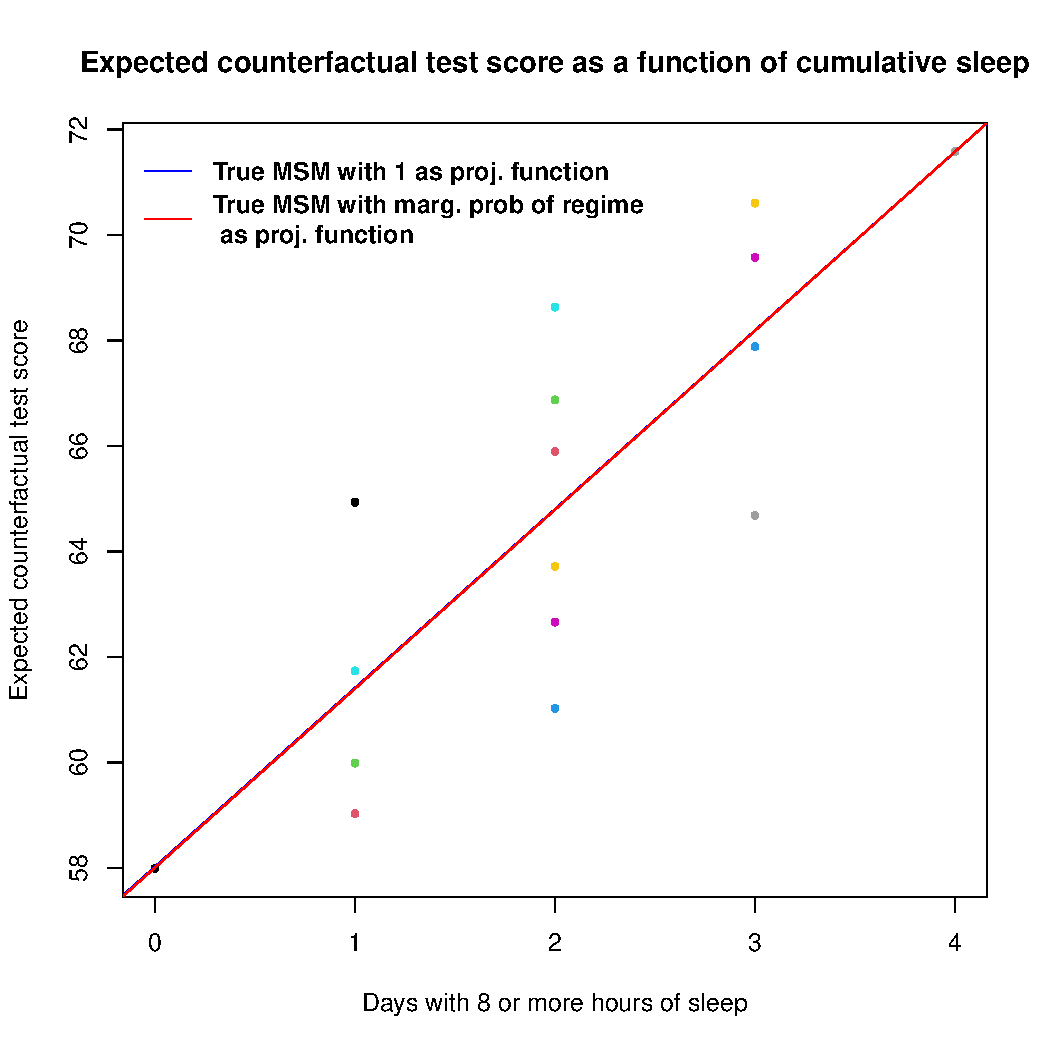
\includegraphics[width=.4\textwidth]{MSM.pdf}
\caption{Plot the true values of expected counterfactual outcomes $E[Y_{\bar{a}}]$ as a function of $\sum_{t = 1}^4 a(t)$ and their corresponding projection onto a linear MSM.  Each of the 16 colored dots represents the expected counterfactual test score of each of the 16 treatment regimes. Both lines are true MSMs; the blue line is the true MSM without weights, and the red line is the true MSM with stabilizing weights. As we can see, the two lines are very similar, meaning that there is little variability in the marginal probabilities for the regimes. Put another way, all of the regimes occur at roughly similar frequencies.
}
\label{Fig:MSM}
\end{center}
\end{myfigure}
\end{solution}



\noindent\large\textbf{Data Structure 3: $O = (L(1), A(1), Y(2), L(2), A(2), Y(3))$}

\normalsize

\noindent\underline{Causal question:} How would the counterfactual probability of becoming sick differ by the time of the test under an intervention to get 8 or more hours of sleep for 2 nights before a statistics test versus an intervention to get less than 8 hours of sleep for 2 nights before a statistics test?

\begin{enumerate}
\item \textbf{Write the causal target parameter that would answer the causal question posed for data structure 3. What are the counterfactual outcomes?} Explain using notation and in words.
\item \textbf{Explain how to intervene on the SCM to get at the causal question/parameter of interest.} Refer back to \texttt{R} Lab 1 for each SCM.
%\item \textbf{Set the seed to 252.}
\item \textbf{Implement the intervention described in step 2} by using \texttt{generate\_data3()} from the previous lab. Call this function \texttt{generate\_data3\_intervene()}.
\item \textbf{Evaluate the causal parameter via simulated counterfactuals.}
\item \textbf{Interpret the estimand you generated in the previous step.}
\end{enumerate}




\pagebreak

\noindent\large\textbf{Data Structure 4: $O = (L(1), C(1), A(1), Y(2), L(2), C(2), A(2), Y(3))$}
\normalsize

\noindent\underline{Causal question:} How would the counterfactual probability of becoming sick differ under an intervention to get 8 or more hours of sleep for 2 nights before a statistics test versus an intervention to get less than 8 hours of sleep for 2 nights before a statistics test, forcing all students to stay in the class for the time of observation?

\begin{enumerate}
\item \textbf{Write the causal target parameter that would answer the causal question posed for data structure 4. What are the counterfactual outcomes?} Explain using notation and in words.
\item \textbf{Explain how to intervene on the SCM to get at the causal question/parameter of interest.} Refer back to \texttt{R} Lab 1 for this data structure's SCM.
%\item \textbf{Set the seed to 252.}
\item \textbf{Implement the intervention described in step 2} by using \texttt{generate\_data4()} from the previous lab. Call this function \texttt{generate\_data4\_intervene()}.
\item \textbf{Evaluate the causal parameter via simulated counterfactuals.}
\item \textbf{Interpret the estimand you generated in the previous step.}
\end{enumerate}



\pagebreak

\section{For Your Project: Evaluating Target Causal Parameters}

Think through the following questions and apply them to the dataset you will use for your final project.

\begin{enumerate}
\item \textbf{Defining your causal question}
\begin{enumerate}
\item What is the causal question (or questions) of interest for your dataset?
\item What is the ideal experiment that would answer your causal question?
\item Which of your variables variables would you intervene on to answer your causal question(s)? What values would you set them equal to?
\item What outcomes are you interested in? Measured when?
\end{enumerate}
\item \textbf{Target parameter and counterfactual outcomes}
\begin{enumerate}
\item What are your counterfactual outcomes, and how would you explain them in words?
\item Come up with a target parameter that would answer your causal question.
\begin{packed_item}
\item[-] What aspects of the counterfactual outcome distribution are you interested in contrasting?
\item[-] What contrast are you interested in (e.g., absolute difference? relative difference? MSMs? conditional on subgroups?)?
\end{packed_item}
\end{enumerate}
\item\textbf{Intervention on SCM}
\begin{enumerate}
\item How would you intervene on the SCM you came up with to evaluate the causal target parameter?
\item Implement this intervention computationally.
\end{enumerate}
\item\textbf{Evaluate $\Psi^F(P_{U,X})$}
\begin{enumerate}
\item Using simulations, generate many counterfactual outcomes.
\item Evaluate $\Psi^F(P_{U,X})$.
\item Write a sentence interpreting your $\Psi^F(P_{U,X})$.
\end{enumerate}
\end{enumerate}


\pagebreak

\section{Feedback}

Please attach responses to these questions to your lab. Thank you in advance!

\begin{enumerate}
\item Did you catch any errors in this lab? If so, where?
\item What did you learn in this lab?
\item Do you think that this lab met the goals listed at the beginning?
\item What else would you have liked to review? What would have helped your understanding?
\item Any other feedback?
\end{enumerate}

\end{document}


